\subsection{Semiconductor detectors}
The measurement were done without any notable incidences, since 
the entire setup is automatized. We saved four data sets:
One for each combination of sample and detector. Due to time constraints, 
the background was not recorded. 

For each data set, we fitted gaussians according to the peaks expected:
For the $\,^{57}$Co sample, we expected two peaks at the right end of a somewhat 
broader distribution of counts with the left one (the 122.06 keV peak) being much higher
then the second (136.47 keV). For the $\,^{241}$Am sample, we expect one peak of 59.5 keV 
(thus roughly at half distance between zero and the $\,^{57}$Co peaks). 
The raw data and fitting is displayed in the panels \ref{fig:detector_CdTe}, 
\ref{fig:detector_Si}.
The fit parameters are listed in the plots. We refrain from stating the entire covariance 
matrices as all further calculations are done with one of the fitted parameters 
each (with the exception of the correspondence energy--channel, which generates new 
errors by linear fitting, loosing the information about correlation). 
The cobalt sample was not very active%
\footnote{an experience we already made during the experiment "short half lives"} 
such that the peak especially for the Si detector had to be done with a very low 
number of data. To be able to observe any signal at all, we rebinned the data 
by using the mean of two successive bins for this data set. In order to have let 
the algorithm converge, we entered initial guesses manually. An experimenting 
with changing initial guesses showed show stability, though . This is not documented 
since we consider the numerical stability of the used algorithms to be 
out of scope. The result of the fitting is, however, very much dependent on the 
range of channels selected to be fitted over. This range is indicated by
the curves of the fits plotted in the above figures. In general, we chose 
a longer range on the right side of each peak, as this side is 
much less influenced by additional underlying distributions. 
Physically, this observation corresponds to the losses during Compton 
scattering or other escaped electrons. In these cases, 
only a part of the entire energy of the initial photon stemming from the decay 
is absorbed by the detector. It is clear that these processes do not influence 
the right (higher energy) side of each peak, as long as overlapping with the next 
peak does not occur. 
\begin{figure}
    \centering
    \begin{subfigure}[b]{\pltw}
        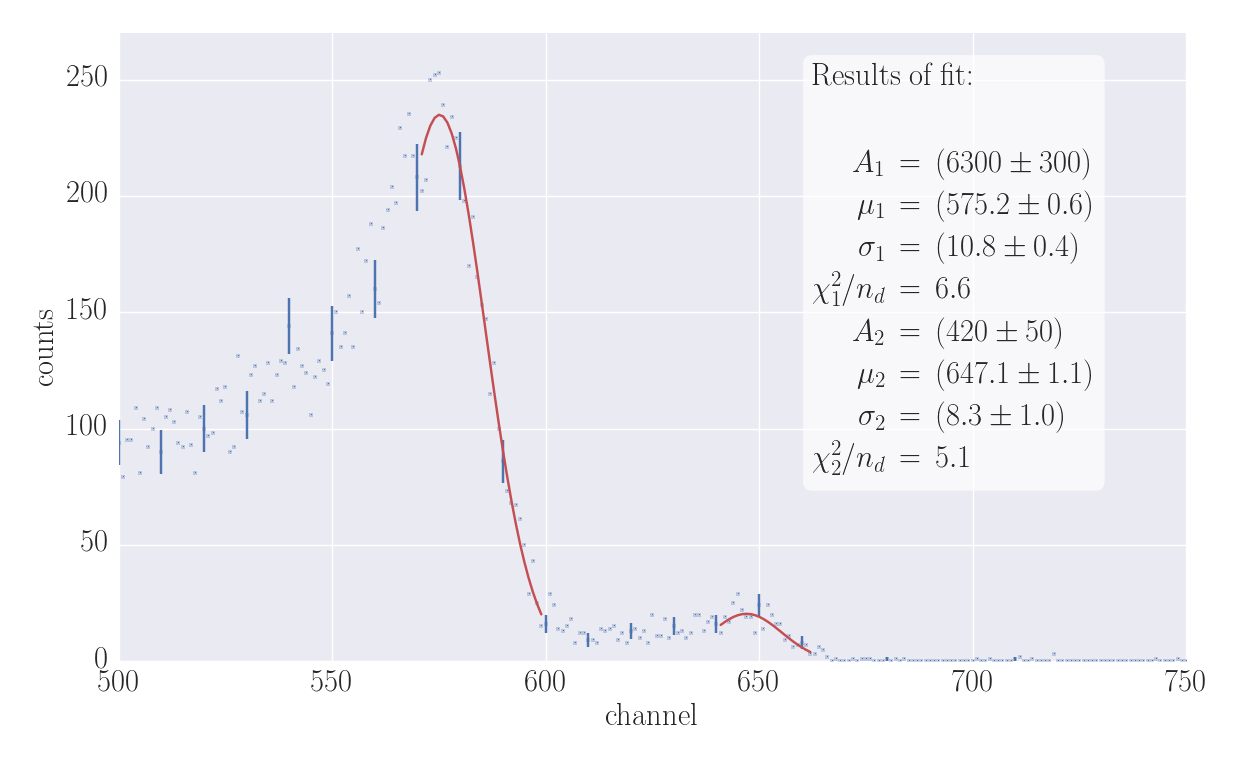
\includegraphics[width=1.0\linewidth]{figures/detector_Co_CdTe}
        \caption{}
        \label{fig:detector_Co_CdTe}
    \end{subfigure}
    \begin{subfigure}[b]{\pltw}
        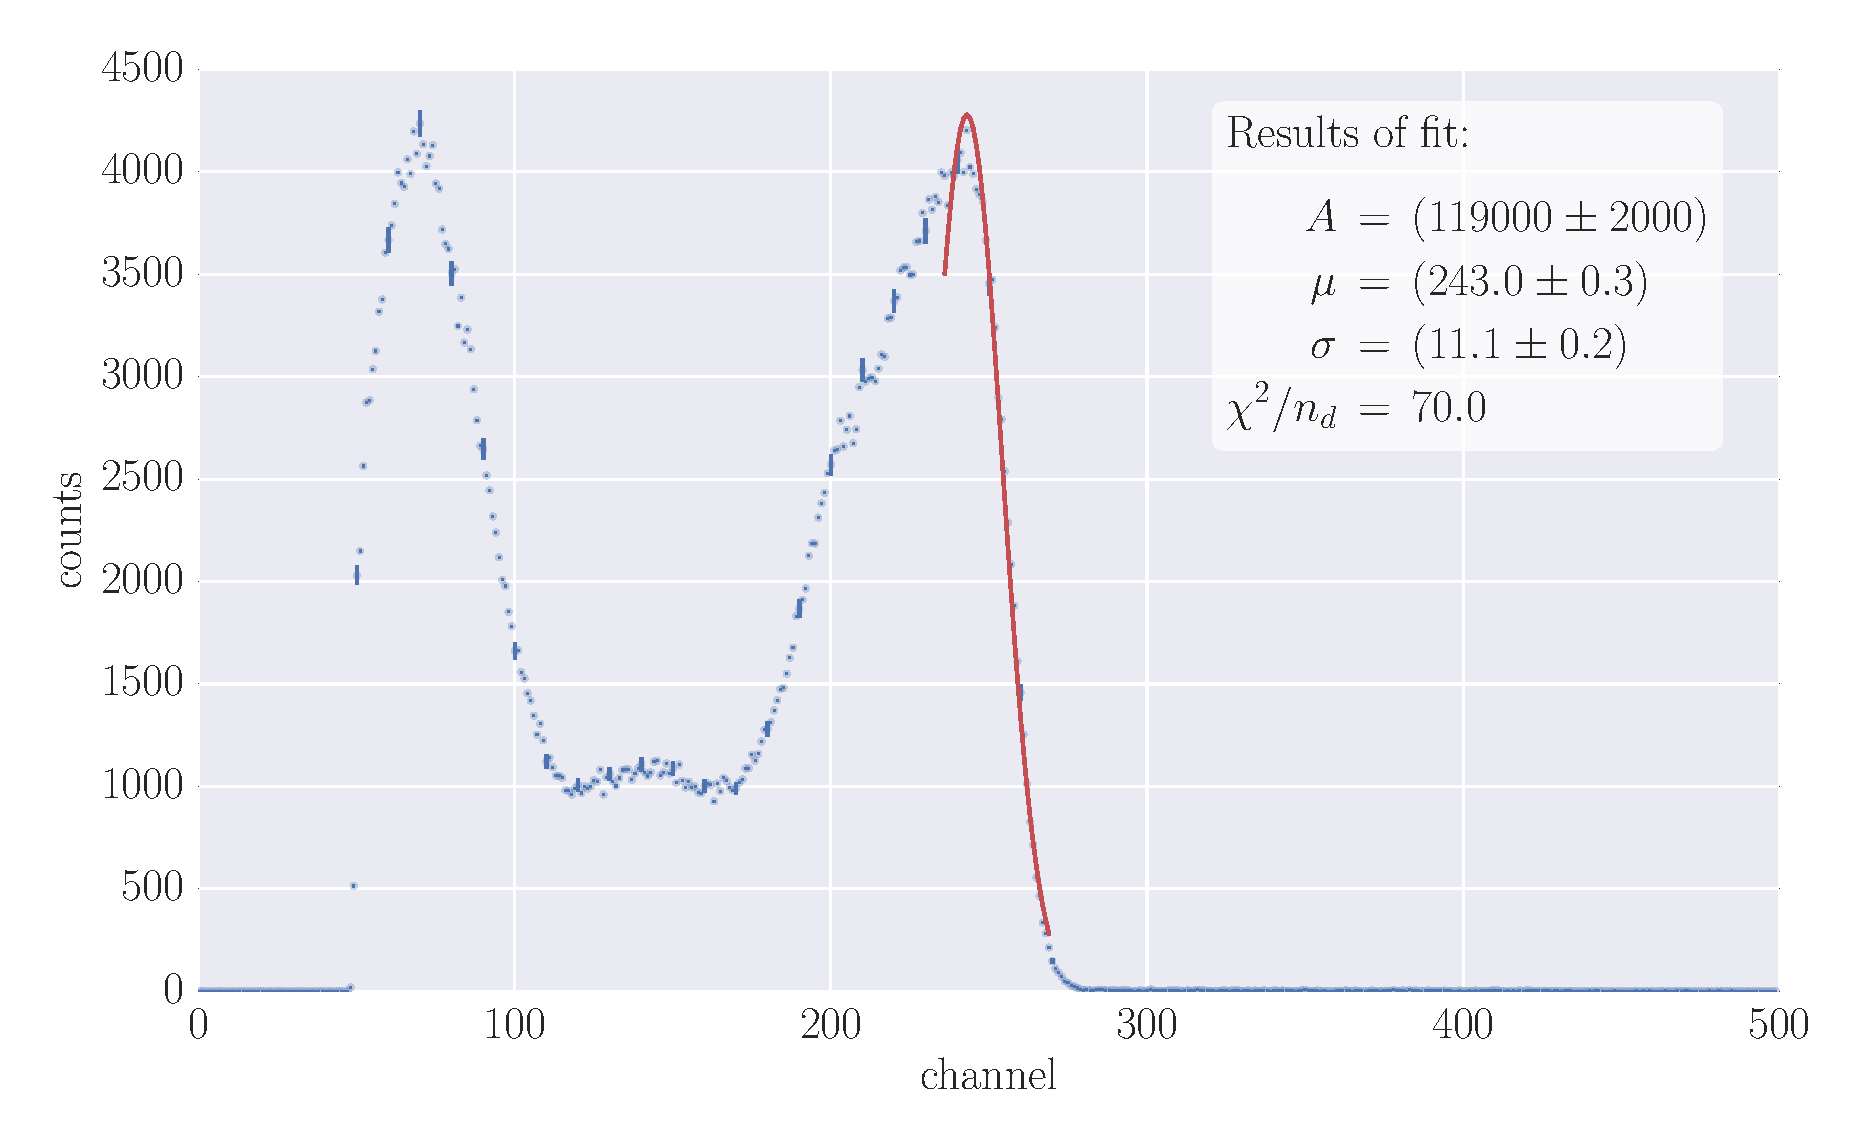
\includegraphics[width=1.0\linewidth]{figures/detector_Am_CdTe}
        \caption{}
        \label{fig:detector_Am_CdTe}
    \end{subfigure}
    \caption{
        Raw data obtained with CdTe detector as well as gaussians fitted 
        onto the expected peaks for the samples $^{57}$Co (\ref{fig:detector_Co_CdTe})
        and $^{241}$Am (\ref{fig:detector_Am_CdTe}). To maintain readability, the error bars 
        are only plotted for every tenth data point. The error is estimated as usual 
        with $\sqrt{N}$, the estimator for random variables following Poisson's distribution. 
        }
    \label{fig:detector_CdTe}
\end{figure}

\begin{figure}
    \centering
    \begin{subfigure}[b]{\pltw}
        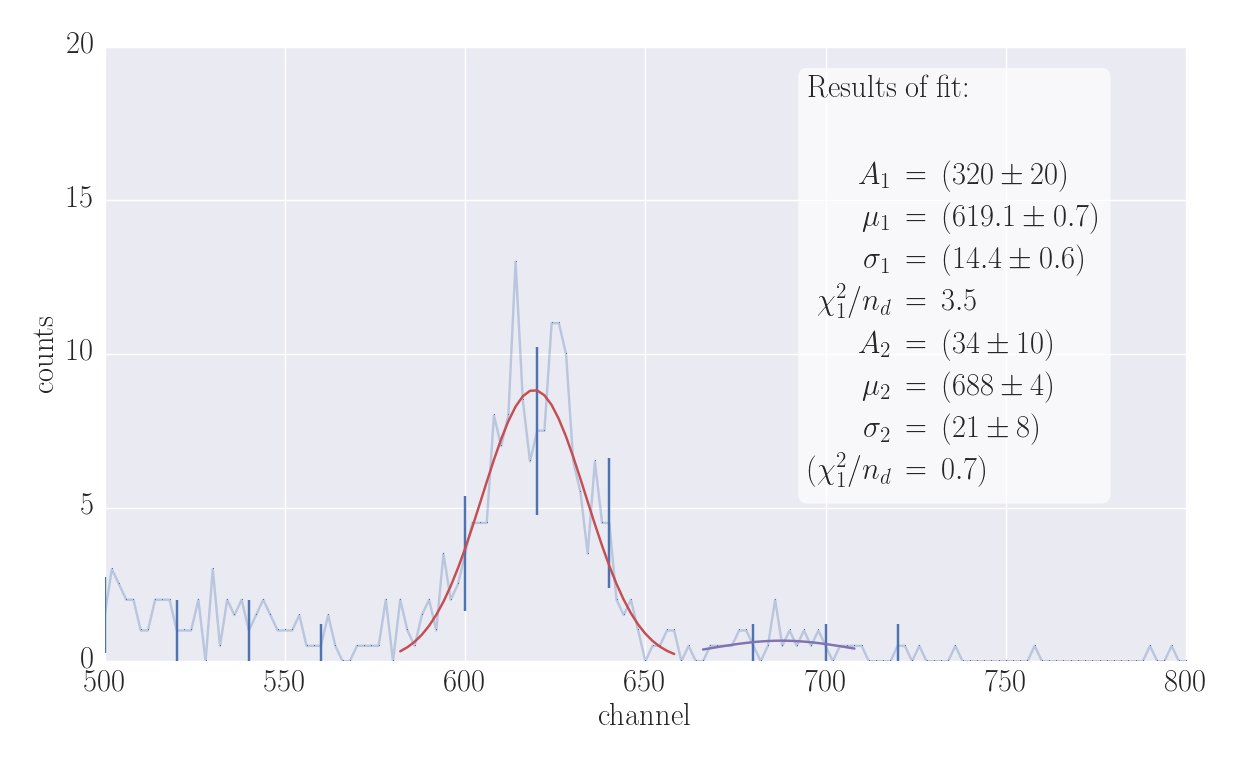
\includegraphics[width=1.0\linewidth]{figures/detector_Co_Si}
        \caption{}
        \label{fig:detector_Co_Si}
    \end{subfigure}
    \begin{subfigure}[b]{\pltw}
        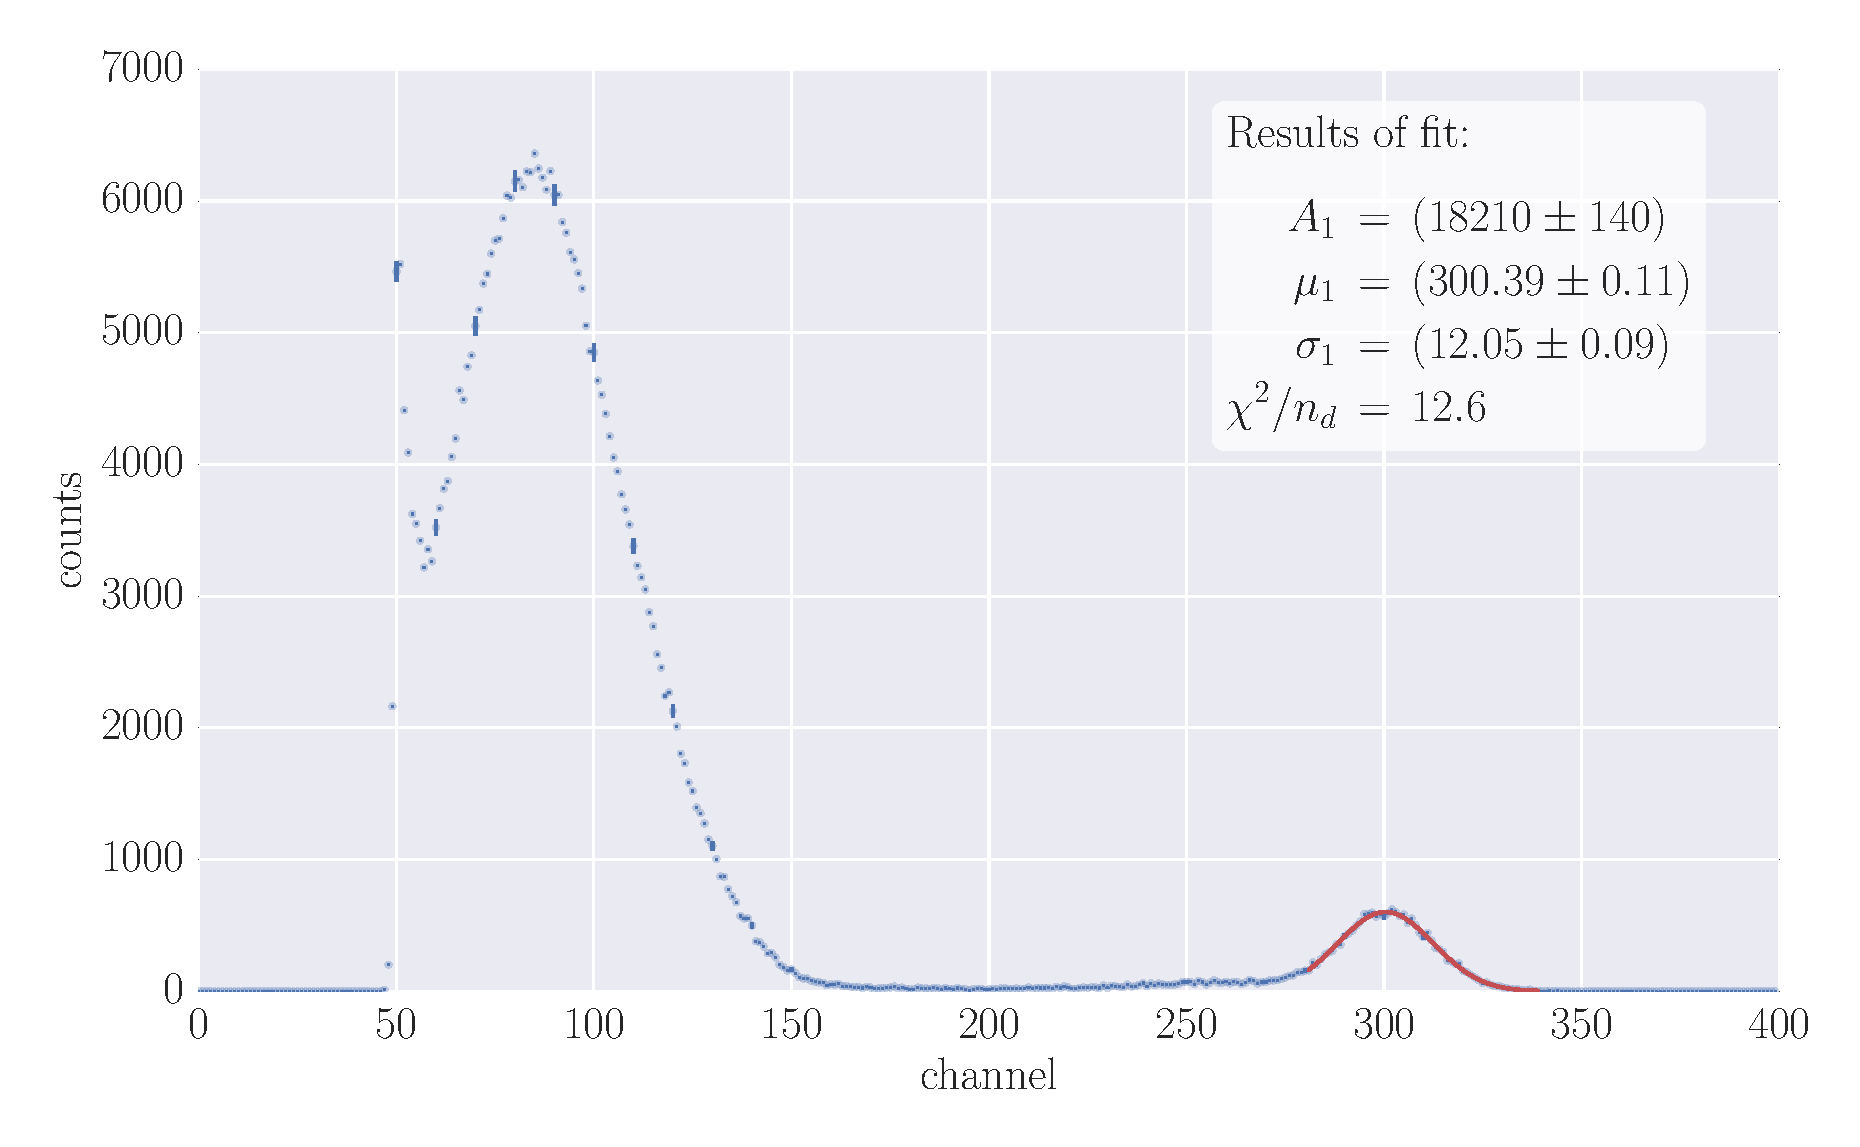
\includegraphics[width=1.0\linewidth]{figures/detector_Am_Si}
        \caption{}
        \label{fig:detector_Am_Si}
    \end{subfigure}
    \caption{
        Raw data obtained with CdTe detector as well as gaussians fitted 
        onto the expected peaks for the samples $^{57}$Co (\ref{fig:detector_Co_CdTe})
        and $^{241}$Am (\ref{fig:detector_Am_CdTe}). The data in the upper plot is rebinned 
        in order to obtain a visible peak.
        }
    \label{fig:detector_Si}
\end{figure}

We take the obtained centers $\mu$ of the distributions to do the calibration, 
i.~e. a linear fit of the form 
\begin{equation}
    E(\mu) = a \mu + E_0 \,
\end{equation}
in order to be able to associate an energy to each peak. The energies 
are taken from the know peaks as described before. The used data is shown in table 
\ref{tab:detector_peaks}, the linear interpolations are plotted in 
figures \ref{fig:detector_calibration}, found in the appendix. We get a linear coefficients
\begin{align}
    a_\mathrm{CdTe}  &=  (0.1890 \pm 0.0011)\, \mathrm{\frac{keV}{ch}}\, \\
    a_\mathrm{Si}  &=  (0.1964  \pm 0.0005)\, \mathrm{\frac{keV}{ch}} \, .
\end{align}
\begin{table}[htdp]
    \centering
    \caption{
        Peaks and corresponding energies for both semiconductors 
        and both samples. The values are used in the linear fit 
        in order to establish the relationship between channel 
        and energy.
        }
    	\begin{tabular}{|p{3cm}|p{3cm}|p{3cm}|p{3cm}|}
		\hline
		\rowcolor{tabcolor}
		Peak   & $E_\mathrm{peak}$ / keV & $\mathrm{\mu_{CdTe}}$ / Channel & $\mathrm{\mu_{Si}}$ / Channel\\ 
		\hline
		$^{241}\mathrm{Am}$ & $59.5$ & $243.0 \pm 0.3$ & $300.39 \pm 0.11$ \\ 
		$^{57}\mathrm{Co}_1$ & $122.06$ & $575.2 \pm 0.6$ & $619.1 \pm 0.7$ \\ 
		$^{57}\mathrm{Co}_2$ & $136.47$ & $647.1 \pm 1.1$ & $688 \pm 4$ \\ 
		\hline
	\end{tabular}

    \label{tab:detector_peaks}
\end{table}
Using these coefficients, we can calculate the relative energy resolution 
of the detectors. This is done applying the formulae discussed in the procedure 
section, see equation \eqref{eq:RER}. The transformation of the standard deviation 
and the resulting resolutions are displayed in table \ref{tab:detector_RER}. 
It turns out that the relative resolution of both detectors lies in the same 
order of magnitude, seeing notable difference only for the 136 keV $^{57}$Co peak.
One has to keep in mind that this peak was especially subject to uncertainties 
as the number of events was to small to do a realistic fit. Further, the Si 
detector has a slightly higher resolution for all tested energies. 
A yet more interesting result of this part of the analysis is, that 
the width of the peaks does not change notably with the energy, 
such that the relative resolution gets better with higher energies. 
In this case, it is about twice as high for the Am peak compared to 
that Co peak for both detectors. 
\begin{table}[htdp]
    \centering
    \caption{
        Relative energy resolutions of CdTe (upper) and 
        Si (lower) detector 
        for the three observed peaks, calculated from the 
        width of the fitted gaussians. 
        }
    	\begin{tabular}{|p{2cm}|p{2.5cm}|p{3cm}|p{3cm}|p{3cm}|}
		\hline
		\rowcolor{tabcolor}
		Peak   & $E_\mathrm{peak}$ / keV & $\sigma_\mathrm{CdTe}$ / Channel &             $\sigma_{E, \mathrm{CdTe}}$ /keV & $\mathrm{RER_{CdTe}}(E)$ \\ 
		\hline
		$^{57}\mathrm{Co}_1$ & $122.06$ & $10.8 \pm 0.4$ & $2.03 \pm 0.07$ & $0.0391 \pm 0.0014$\\ 
		$^{57}\mathrm{Co}_2$ & $136.47$ & $8.3 \pm 1.0$ & $1.6 \pm 0.2$ & $0.027 \pm 0.003$\\ 
		$^{241}\mathrm{Am}$ & $59.5$ & $11.1 \pm 0.2$ & $2.10 \pm 0.04$ & $0.083 \pm 0.002$\\ 
		\hline &&&&\\ 
		\hline
		\rowcolor{tabcolor}
		Peak   & $E_\mathrm{peak}$ / keV & $\sigma_\mathrm{Si}$ / Channel &             $\sigma_{E, \mathrm{Si}}$ /keV & $\mathrm{RER_{Si}}(E)$ \\ 
		\hline
		$^{57}\mathrm{Co}_1$ & $122.06$ & $10.8 \pm 0.4$ & $2.03 \pm 0.07$ & $0.0391 \pm 0.0014$\\ 
		$^{57}\mathrm{Co}_2$ & $136.47$ & $8.3 \pm 1.0$ & $1.6 \pm 0.2$ & $0.027 \pm 0.003$\\ 
		$^{241}\mathrm{Am}$ & $59.5$ & $11.1 \pm 0.2$ & $2.10 \pm 0.04$ & $0.083 \pm 0.002$\\ 
		\hline
	\end{tabular}

    \label{tab:detector_RER}
\end{table}
The crucial part of this experiment lies in analyzing the qualities 
of both semiconductors as detectors, which is quantitatively expressed 
by the absorption probability: In many occasions one wants to now the 
activity of a sample. In order to get reliable data, it is crucial to 
register as many emitted photons as possible -- thus a higher absorption 
coefficient indicates a better material for the according experiments. 
We expect the CdTe semiconductor to show a much higher absorption rate 
due to its higher mass density (which is a determining factor for the 
    cross section). 
\begin{table}[htdp]
    \centering
    \caption{
        Amplitudes $A$ obtained from the gaussian fits and 
        resulting absorption ratio between CdTe and Si detector 
        with the active areas $a_{Si} = 100\, \mathrm{mm^2}$ and 
        $a_{CdTe} = 23\, \mathrm{mm^2}$.
        }
    	\begin{tabular}{|p{3cm}|p{3cm}|p{3cm}|p{3cm}|}
		\hline
		\rowcolor{tabcolor}
		Peak   & $A_\mathrm{CdTe}$ & $A_\mathrm{Si}$ & $P$\\ 
		\hline
		$^{57}\mathrm{Co}_1$ & $6300 \pm 300$ & $320 \pm 20$ & $0.219 \pm 0.014$\\ 
		$^{57}\mathrm{Co}_2$ & $420 \pm 50$ & $34 \pm 10$ & $0.35 \pm 0.11$\\ 
		$^{241}\mathrm{Am}$ & $119000 \pm 2000$ & $18210 \pm 140$ & $0.664 \pm 0.014$\\ 
		\hline
	\end{tabular}

    \label{tab:detector_ratio}
\end{table}
The literature values~\cite{nist} for the energies under 
examination are given by 
\begin{align}
    \frac{A_\mathrm{Si}}{A_\mathrm{CdTe}}(59 \,\mathrm{keV}) &= 1.40 \% \\
    \frac{A_\mathrm{Si}}{A_\mathrm{CdTe}}(122 \,\mathrm{keV}) &= 1.83 \% \\
    \frac{A_\mathrm{Si}}{A_\mathrm{CdTe}}(136 \,\mathrm{keV}) &= 2.00 \%
\end{align}
The order of magnitude is correct in all cases, although 
errors obtained from propagation underestimate the 
real errors -- due to the low number of data as well as systematic 
errors introduced for example by the different losses. 
The obtained values do not quite show the expected behavior 
of rising absorption ratio for higher energies.
However, 
it is clear, that the CdTe has a much higher absorption coefficient and 
can thus be considered to be the better detector in this kind of 
experiment. 
